% =============================================================================
% CAPÍTULO 6 — CONFIGURACIÓN AVANZADA, SEGURIDAD E INTEGRACIÓN DE HARDWARE
% =============================================================================
\chapter[Configuración, Seguridad y Hardware]{Configuración Avanzada, Seguridad e Integración de Hardware}%
\label{ch:seguridad}
\resumenCapitulo{Este capítulo aborda la configuración de seguridad del despliegue en tres
planos: las políticas del servidor de recursos (validación de JWT y cabeceras de
seguridad), el control de acceso en la capa de datos (RLS y custodia de la clave de
servicio) y, de forma destacada, el procedimiento literal para habilitar el acceso a
cámara y micrófono de la PWA en entornos HTTP sin certificado, navegador por navegador.}

La seguridad de EthosHub se asienta en tres capas complementarias. La primera vive en el
\textbf{backend}, que actúa como servidor de recursos y valida cada credencial. La segunda
vive en la \textbf{base de datos}, donde las políticas RLS aíslan los datos de cada
usuario. La tercera afecta al \textbf{cliente}, donde el navegador impone restricciones a
las funciones de hardware (cámara/micrófono) cuando el origen no es seguro. Este capítulo
las cubre en ese orden.\par

% -----------------------------------------------------------------------------
\section[Políticas del Servidor de Recursos]{Configuración de Políticas de Seguridad del Servidor de Recursos (Resource Server)}%
\label{sec:resource-server}

El backend no emite credenciales: las \textbf{valida}. Opera como un \textit{Resource
Server} OAuth2 que confía en los \textit{tokens} firmados por Supabase Auth.\par

\subsection[Validación de Tokens JWT de Supabase]{Validación de Tokens de Acceso Firmados (JWT) Emitidos por Supabase}%
\label{subsec:jwt}

Cada petición protegida debe portar un JWT en la cabecera \comando{Authorization: Bearer
<token>}. El backend verifica la firma del \textit{token} contra el JWKS de Supabase, cuya
URL se configura mediante la propiedad \comando{jwk-set-uri} (variable de entorno
\comando{SUPABASE\_JWK\_SET\_URI}). La figura~\ref{fig:jwt} resume el flujo de validación.\par

\vspace{0.3cm}
\begin{figure}[h!]
\centering
\begin{tikzpicture}[node distance=0.6cm and 1.4cm, every node/.style={font=\sffamily\scriptsize}]
    \node[c4persona, minimum width=2.0cm, minimum height=0.9cm] (cli) {Cliente};
    \node[c4sistema, right=of cli, minimum width=2.4cm, minimum height=0.9cm] (be) {Backend\\\scriptsize Resource Server};
    \node[c4externo, right=of be, minimum width=2.2cm, minimum height=0.9cm] (jwks) {Supabase\\\scriptsize JWKS};
    \draw[c4flecha] (cli) -- node[c4etiqueta, above]{Bearer JWT} (be);
    \draw[c4flecha] (be) -- node[c4etiqueta, above]{clave pública} (jwks);
    \draw[c4flecha] (be.south) to[bend right=25] node[c4etiqueta, below]{200 / 401} (cli.south);
\end{tikzpicture}
\caption{Validación de JWT: el backend obtiene la clave pública del JWKS de Supabase y verifica la firma del token.}%
\label{fig:jwt}
\end{figure}

\begin{lstlisting}[language=bash]
# application-prod.yml (extracto)
spring:
  security:
    oauth2:
      resourceserver:
        jwt:
          jwk-set-uri: ${SUPABASE_JWK_SET_URI}
\end{lstlisting}

\begin{VerificacionOK}
Una petición sin \textit{token} o con un \textit{token} inválido recibe \textbf{401
Unauthorized}; una petición autenticada pero sin permisos recibe \textbf{403 Forbidden}.
Estos códigos los normaliza el \comando{GlobalExceptionHandler} y se verifican en el
apartado~\ref{subsec:401-403}.
\end{VerificacionOK}

\subsection[Filtro de Cabeceras de Seguridad]{Configuración del Filtro de Cabeceras de Seguridad (\texttt{Security\-Headers\-Filter})}%
\label{subsec:headers}

El paquete \comando{config/} del backend registra varios filtros propios. Entre ellos, el
\comando{SecurityHeadersFilter} añade cabeceras de protección a cada respuesta; junto a él
operan \comando{CookieTokenFilter} (lee el \textit{token} desde una \textit{cookie}),
\comando{NoCacheFilter} y \comando{SpaFallbackFilter}. La tabla~\ref{tab:filtros} los
resume.\par

\vspace{0.2cm}
\noindent
\renewcommand{\arraystretch}{1.35}
\fontsize{8.7}{10.4}\selectfont\sffamily
\begin{tabularx}{\dimexpr\textwidth-2pt\relax}{|>{\ttfamily\bfseries\color{colorPrimario}}l|X|}
\hline
\rowcolor{headerTabla}
\sffamily\textbf{Filtro} & \sffamily\textbf{Función} \\
\hline
SecurityHeadersFilter & Inyecta cabeceras de seguridad (anti-\textit{clickjacking}, tipo de contenido, etc.). \\
\hline
\rowcolor{grisTecnico}
CookieTokenFilter & Extrae el JWT desde una \textit{cookie} si no viaja en la cabecera. \\
\hline
NoCacheFilter & Evita el cacheo de respuestas sensibles. \\
\hline
\rowcolor{grisTecnico}
SpaFallbackFilter & Sirve \texttt{index.html} para las rutas de la SPA (enrutamiento cliente). \\
\hline
\end{tabularx}\normalfont\normalsize%
\label{tab:filtros}

\begin{NotaConfiguracion}
Estos filtros funcionan sin configuración adicional del operador: se activan al arrancar
el JAR. La política \comando{AdminEmailPolicy} restringe las operaciones administrativas a
las cuentas \comando{adm.*@ethoshub.dev} y \comando{admin@ethoshub.dev}; si necesita
habilitar un administrador distinto, esa política debe ajustarse en el código antes de
empaquetar.
\end{NotaConfiguracion}

% -----------------------------------------------------------------------------
\section[Control de Acceso en la Capa de Datos]{Aprovisionamiento de Políticas de Control de Acceso en la Capa de Datos}%
\label{sec:control-datos}

La segunda capa de defensa reside en PostgreSQL. Aunque un atacante eludiera la API, las
políticas de la base de datos seguirían restringiendo el acceso a las filas.\par

\subsection[Seguridad Basada en Filas (RLS)]{Configuración de la Seguridad Basada en Filas (Row Level Security -- RLS) en Supabase}%
\label{sec:rls}

La \textbf{Row Level Security} (RLS) restringe, fila a fila, qué registros puede leer o
modificar cada usuario según su identidad. En EthosHub, las migraciones que aprovisionó en
el apartado~\ref{subsec:migraciones} crean estas políticas sobre las tablas del esquema
\comando{core}. Las operaciones que deben actuar por encima de RLS (por ejemplo, ciertas
acciones administrativas) se canalizan mediante RPCs \comando{SECURITY DEFINER}, que se
ejecutan con los privilegios de su propietario sin desactivar globalmente la seguridad.\par

El listado siguiente muestra el patrón de una política RLS típica del esquema
\comando{core}: cada usuario solo accede a las filas cuyo \comando{user\_id} coincide con
su identidad autenticada (\comando{auth.uid()}).\par

\begin{lstlisting}[language=bash]
-- Activar RLS sobre la tabla y declarar la politica de aislamiento por usuario
ALTER TABLE core.projects ENABLE ROW LEVEL SECURITY;

CREATE POLICY projects_owner_select ON core.projects
    FOR SELECT USING (auth.uid() = user_id);

CREATE POLICY projects_owner_modify ON core.projects
    FOR ALL USING (auth.uid() = user_id) WITH CHECK (auth.uid() = user_id);
\end{lstlisting}

\begin{AvisoAdvertencia}
\textbf{Nunca demote el rol dentro de una función \texttt{SECURITY DEFINER}} ni desactive
RLS «temporalmente» en producción para depurar. Hacerlo expone los datos de todos los
usuarios. Si una consulta no devuelve los datos esperados, el diagnóstico correcto es
revisar la política RLS aplicable, no deshabilitarla.
\end{AvisoAdvertencia}

\subsubsection{Configuración de CORS para despliegues de origen separado}
En el monolito, cliente y API son \textit{same-origin} y CORS es irrelevante. Si, en
cambio, sirve el \textit{frontend} desde un dominio distinto al backend, debe declarar los
orígenes permitidos en la variable \comando{CORS\_ALLOWED\_ORIGINS}; el componente
\comando{CorsConfig} del paquete \comando{config/} la consume.\par

\begin{lstlisting}[language=bash]
# Solo necesario si FE y BE estan en dominios distintos
CORS_ALLOWED_ORIGINS=https://app.bytebusters.com,https://bytebusters.tis.cs.umss.edu.bo
\end{lstlisting}

\begin{NotaConfiguracion}
Mantenga \comando{CORS\_ALLOWED\_ORIGINS} lo más restrictiva posible: enumere únicamente
los orígenes legítimos. Evite el comodín \comando{*} en producción, pues permitiría que
cualquier sitio consumiera la API en nombre del usuario autenticado.
\end{NotaConfiguracion}

\subsection[Custodia de la \texttt{SERVICE\_ROLE\_KEY}]{Restricción de Roles Críticos y Almacenamiento Seguro de la \texttt{SERVICE\_\-ROLE\_\-KEY}}%
\label{subsec:servicerole}

La \comando{SUPABASE\_SERVICE\_ROLE\_KEY} es la credencial más sensible del sistema:
otorga acceso total a la base de datos \textbf{saltándose RLS}. Su custodia se rige por las
reglas de la tabla~\ref{tab:custodia}.\par

\vspace{0.2cm}
\noindent
\renewcommand{\arraystretch}{1.35}
\fontsize{8.7}{10.4}\selectfont\sffamily
\begin{tabularx}{\dimexpr\textwidth-2pt\relax}{|>{\bfseries\color{colorPrimario}}l|X|}
\hline
\rowcolor{headerTabla}
\textbf{Regla} & \textbf{Detalle} \\
\hline
Solo backend & La clave se inyecta como variable de entorno del servidor; jamás en \texttt{VITE\_*}. \\
\hline
\rowcolor{grisTecnico}
Nunca en el cliente & No debe aparecer en el \textit{bundle} JavaScript ni en el navegador. \\
\hline
Fuera del control de versiones & \texttt{application-prod.yml} está ignorado por git; use \texttt{.env} o secretos del orquestador. \\
\hline
\rowcolor{grisTecnico}
Rotación tras exposición & Si se filtró (incluido el historial de git), debe rotarse de inmediato. \\
\hline
\end{tabularx}\normalfont\normalsize%
\label{tab:custodia}

\begin{AlertaSeguridad}
Confunda la \comando{ANON\_KEY} con la \comando{SERVICE\_ROLE\_KEY} y comprometerá toda la
base de datos. Regla mnemotécnica: la \textbf{anon} es \textbf{pública} (va al navegador,
protegida por RLS); la \textbf{service-role} es \textbf{secreta} (solo el servidor, ignora
RLS). Verifique, antes de cada despliegue, que ninguna variable \comando{VITE\_*} contiene
la palabra \comando{service}.
\end{AlertaSeguridad}

% -----------------------------------------------------------------------------
\section[Excepciones PWA en HTTP (Cámara y Micrófono)]{Excepciones de Seguridad PWA en Entornos Inseguros HTTP (Uso de Cámara y Micrófono)}%
\label{sec:pwa-http}

Las funcionalidades avanzadas de captura de vídeo y audio en el módulo del estudio de
currículums y entrevistas dependen directamente de la API WebRTC (\comando{react-webcam}).
Por diseño de seguridad industrial, los navegadores modernos restringen el acceso a
dispositivos de hardware a menos que la aplicación sea servida bajo un origen seguro
(\comando{https://} o \comando{localhost}).\par

Cuando el despliegue se realiza en una red local o un subdominio institucional sin
certificado válido, se debe aplicar el siguiente procedimiento técnico en las estaciones
de trabajo o dispositivos móviles de los perfiles que evalúan el sistema, con la finalidad
de añadir los orígenes de confianza de forma explícita. La figura~\ref{fig:flag-mockup}
ilustra el aspecto de la pantalla de banderas de un navegador basado en Chromium una vez
configurada.\par

\subsubsection{Paso previo: identificación del origen a declarar}
Antes de tocar ningún navegador, determine \textbf{exactamente} el origen bajo el cual los
usuarios acceden a la aplicación. Un \textit{origen} es la terna \comando{esquema://host:puerto}
y debe declararse \textbf{tal cual} aparece en la barra de direcciones, sin barra final. En
el despliegue de evaluación de EthosHub son dos:\par

\begin{itemize}[noitemsep]
    \item \dir{http://192.168.100.23:3000} — acceso por IP en la red local (puerto 3000 en desarrollo; use el puerto real del despliegue).
    \item \dir{http://bytebusters.tis.cs.umss.edu.bo} — acceso por el subdominio institucional.
\end{itemize}

Si desconoce la IP del servidor, obténgala con \comando{ip addr} (Linux) o
\comando{ipconfig} (Windows). En la lista de orígenes del navegador, \textbf{ambos} se
escriben separados por una coma, sin espacios:\par

\begin{lstlisting}[basicstyle=\ttfamily\small,numbers=none,frame=single,backgroundcolor=\color{grisTecnico}]
http://192.168.100.23:3000,http://bytebusters.tis.cs.umss.edu.bo
\end{lstlisting}

\begin{AvisoPrecaucion}
El origen debe coincidir \textbf{carácter a carácter} con el de la barra de direcciones. Un
puerto distinto (\dir{:3000} frente a \dir{:8080}), \comando{http} frente a \comando{https},
o una IP cambiada por DHCP invalidan la excepción. Si el servidor obtiene su IP por DHCP,
fíjela (reserva estática) para que el origen declarado no deje de ser válido.
\end{AvisoPrecaucion}

\vspace{0.3cm}
\begin{figure}[h!]
\centering
\begin{tikzpicture}[font=\sffamily\scriptsize]
    % Marco de ventana del navegador
    \fill[chromeBar, rounded corners=3pt] (0,0) rectangle (12,3.4);
    \fill[chromeField, rounded corners=2pt] (0.3,2.7) rectangle (9.0,3.2);
    \node[anchor=west, font=\ttfamily\scriptsize] at (0.4,2.95) {chrome://flags/\#unsafely-treat-insecure-origin-as-secure};
    % Tarjeta de la bandera
    \fill[white, rounded corners=3pt] (0.3,0.3) rectangle (11.7,2.4);
    \node[anchor=west, font=\sffamily\bfseries] at (0.5,2.0) {Insecure origins treated as secure};
    \node[anchor=west, text width=8.2cm, font=\sffamily\scriptsize, color=grisISO] at (0.5,1.4)
        {Treat given (insecure) origins as secure origins. Separe múltiples orígenes con comas.};
    % Campo de orígenes
    \fill[chromeField, draw=grisISO!50, rounded corners=2pt] (0.5,0.5) rectangle (11.4,0.95);
    \node[anchor=west, font=\ttfamily\tiny] at (0.6,0.72) {http://192.168.100.23:3000,http://bytebusters.tis.cs.umss.edu.bo};
    % Selector Enabled
    \fill[flagEnabled, rounded corners=3pt] (9.6,1.0) rectangle (11.5,1.6);
    \node[white, font=\sffamily\bfseries] at (10.55,1.3) {Enabled};
\end{tikzpicture}
\caption{Aspecto de la bandera «Insecure origins treated as secure» configurada en un navegador Chromium, con los orígenes de confianza declarados y el selector en \textit{Enabled}.}%
\label{fig:flag-mockup}
\end{figure}

\begin{AlertaSeguridad}
Las banderas descritas a continuación \textbf{reducen deliberadamente la seguridad} del
navegador y deben aplicarse \textbf{únicamente} en los equipos de evaluación, frente a los
dominios de prueba del proyecto. Revierta estos cambios al finalizar la evaluación
(capítulo~\ref{ch:desinstalacion}). La solución definitiva es servir la aplicación bajo
HTTPS con un certificado válido.
\end{AlertaSeguridad}

\subsection[Google Chrome (Escritorio y Android)]{Configuración del Motor Chromium en Entornos de Escritorio y Android (Google Chrome)}%
\label{subsec:chrome}

El navegador Google Chrome emplea la misma arquitectura de banderas de desarrollo tanto en
entornos de escritorio como en su distribución móvil para el sistema operativo Android. El
procedimiento es análogo, pero la ubicación de los controles difiere; por ello se detalla
cada plataforma por separado.\par

\paragraph{En computadora de escritorio (Windows, macOS, Linux).}
\begin{enumerate}[noitemsep]
    \item Abra Google Chrome y haga clic en la barra de direcciones superior.
    \item Escriba la siguiente dirección de configuración interna y pulse \textit{Enter}:\par
    \dir{chrome://flags/\#unsafely-treat-insecure-origin-as-secure}
    \item La página de banderas se abre con la opción \textbf{«Insecure origins treated as secure»} resaltada en amarillo.
    \item En el desplegable a la derecha de esa opción, cambie el valor de \textit{Disabled} (o \textit{Default}) a \textbf{Enabled}.
    \item En el cuadro de texto que se habilita justo debajo, escriba los orígenes exactos separados por comas (sin espacios):\par
    \dir{http://192.168.100.23:3000,http://bytebusters.tis.cs.umss.edu.bo}
    \item Pulse el botón azul \textbf{Relaunch} (Reiniciar) que aparece abajo a la derecha. Chrome se reinicia conservando las pestañas.
    \item Vuelva a abrir la aplicación: el origen ya se trata como seguro.
\end{enumerate}

\begin{figure}[htbp]
\centering
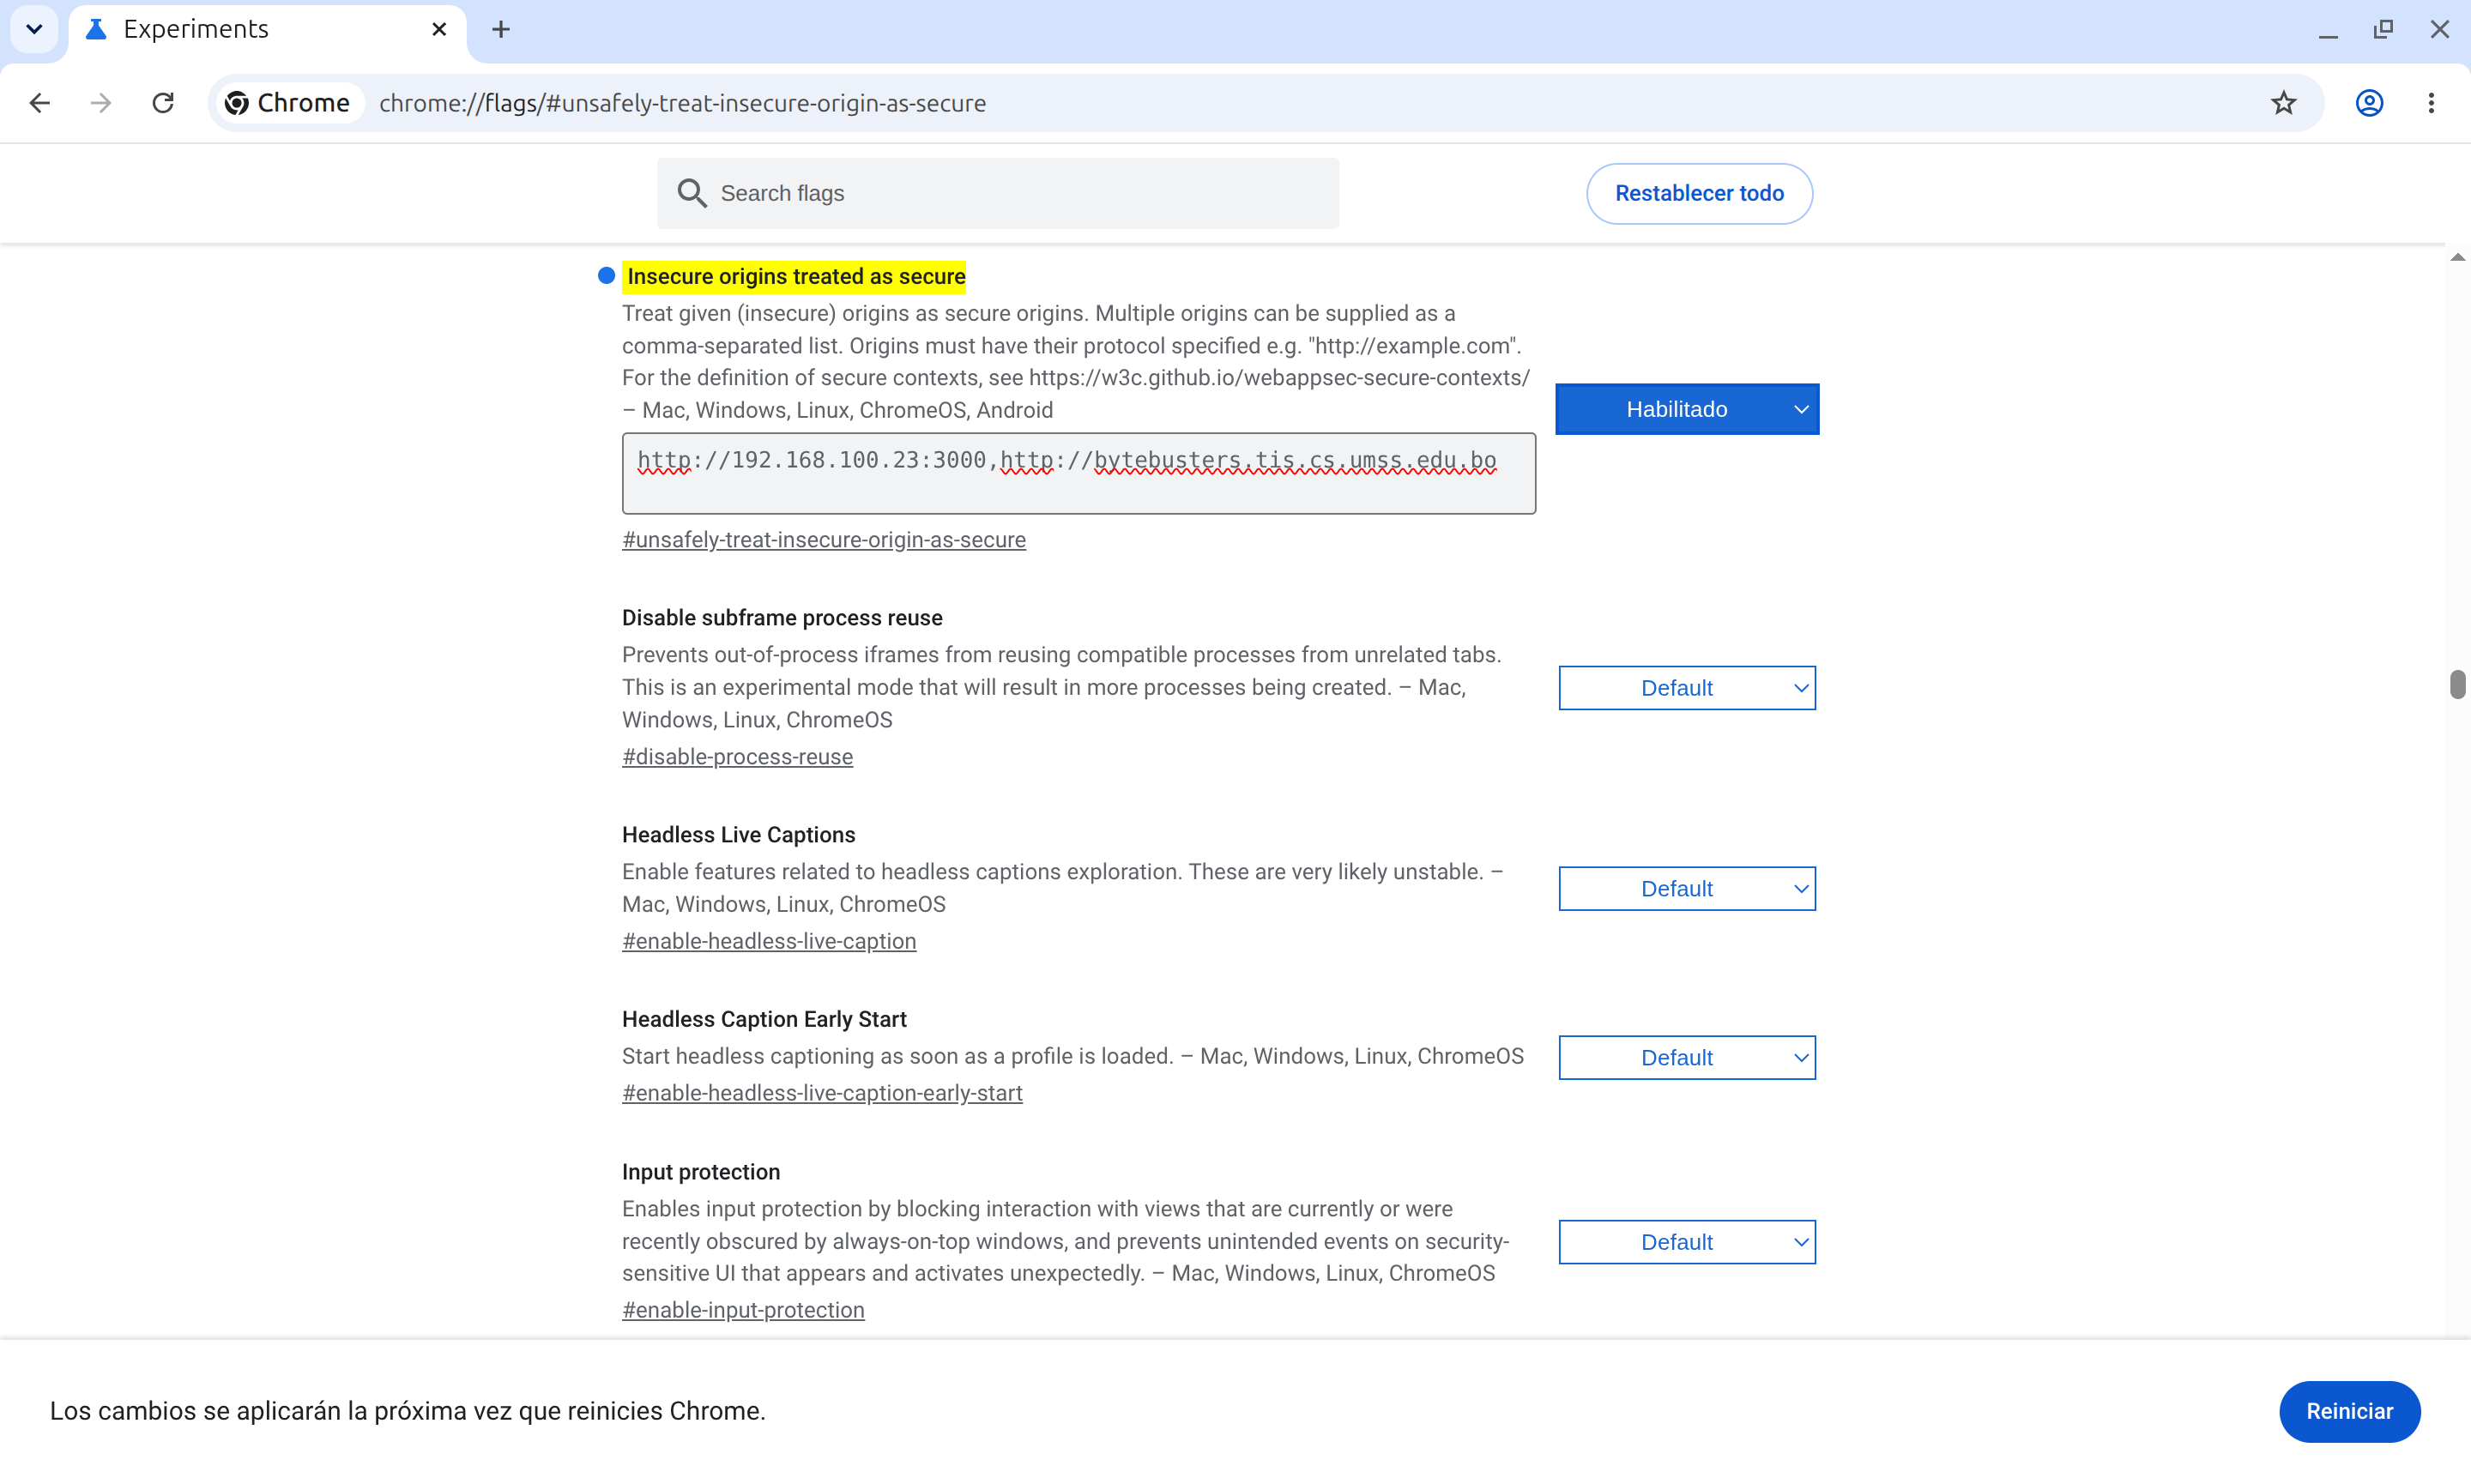
\includegraphics[width=0.85\linewidth]{assets/img/ethoshub/chrome_pc.png}
\caption{Página \texttt{chrome://flags} en Google Chrome de escritorio, con la bandera «Insecure origins treated as secure» en \textit{Enabled} y los orígenes de confianza declarados.}%
\label{fig:chrome-pc-flag}
\end{figure}

\paragraph{En teléfono o tableta Android.}
\begin{enumerate}[noitemsep]
    \item Abra la app de Google Chrome en el dispositivo Android.
    \item Toque la barra de direcciones (arriba) y escriba la dirección de banderas; toque «Ir»:\par
    \dir{chrome://flags/\#unsafely-treat-insecure-origin-as-secure}
    \item Use el buscador de la parte superior de la página de banderas y escriba \comando{insecure} para localizar rápidamente la opción \textbf{«Insecure origins treated as secure»}.
    \item Toque el desplegable bajo esa opción y seleccione \textbf{Enabled}.
    \item Toque el campo de texto que aparece e ingrese los mismos orígenes separados por comas (sin espacios):\par
    \dir{http://192.168.100.23:3000,http://bytebusters.tis.cs.umss.edu.bo}
    \item Toque el botón \textbf{Relaunch} que surge en la parte inferior de la pantalla para reiniciar Chrome en Android.
    \item Al volver a la aplicación, Android \textbf{además} pedirá permiso de cámara/micrófono mediante un diálogo del sistema: toque \textbf{Permitir}. Si lo rechazó antes, habilítelo en \comando{Ajustes} $\to$ \comando{Aplicaciones} $\to$ \comando{Chrome} $\to$ \comando{Permisos}.
\end{enumerate}

\clearpage
\begin{figure}[htbp]
\centering
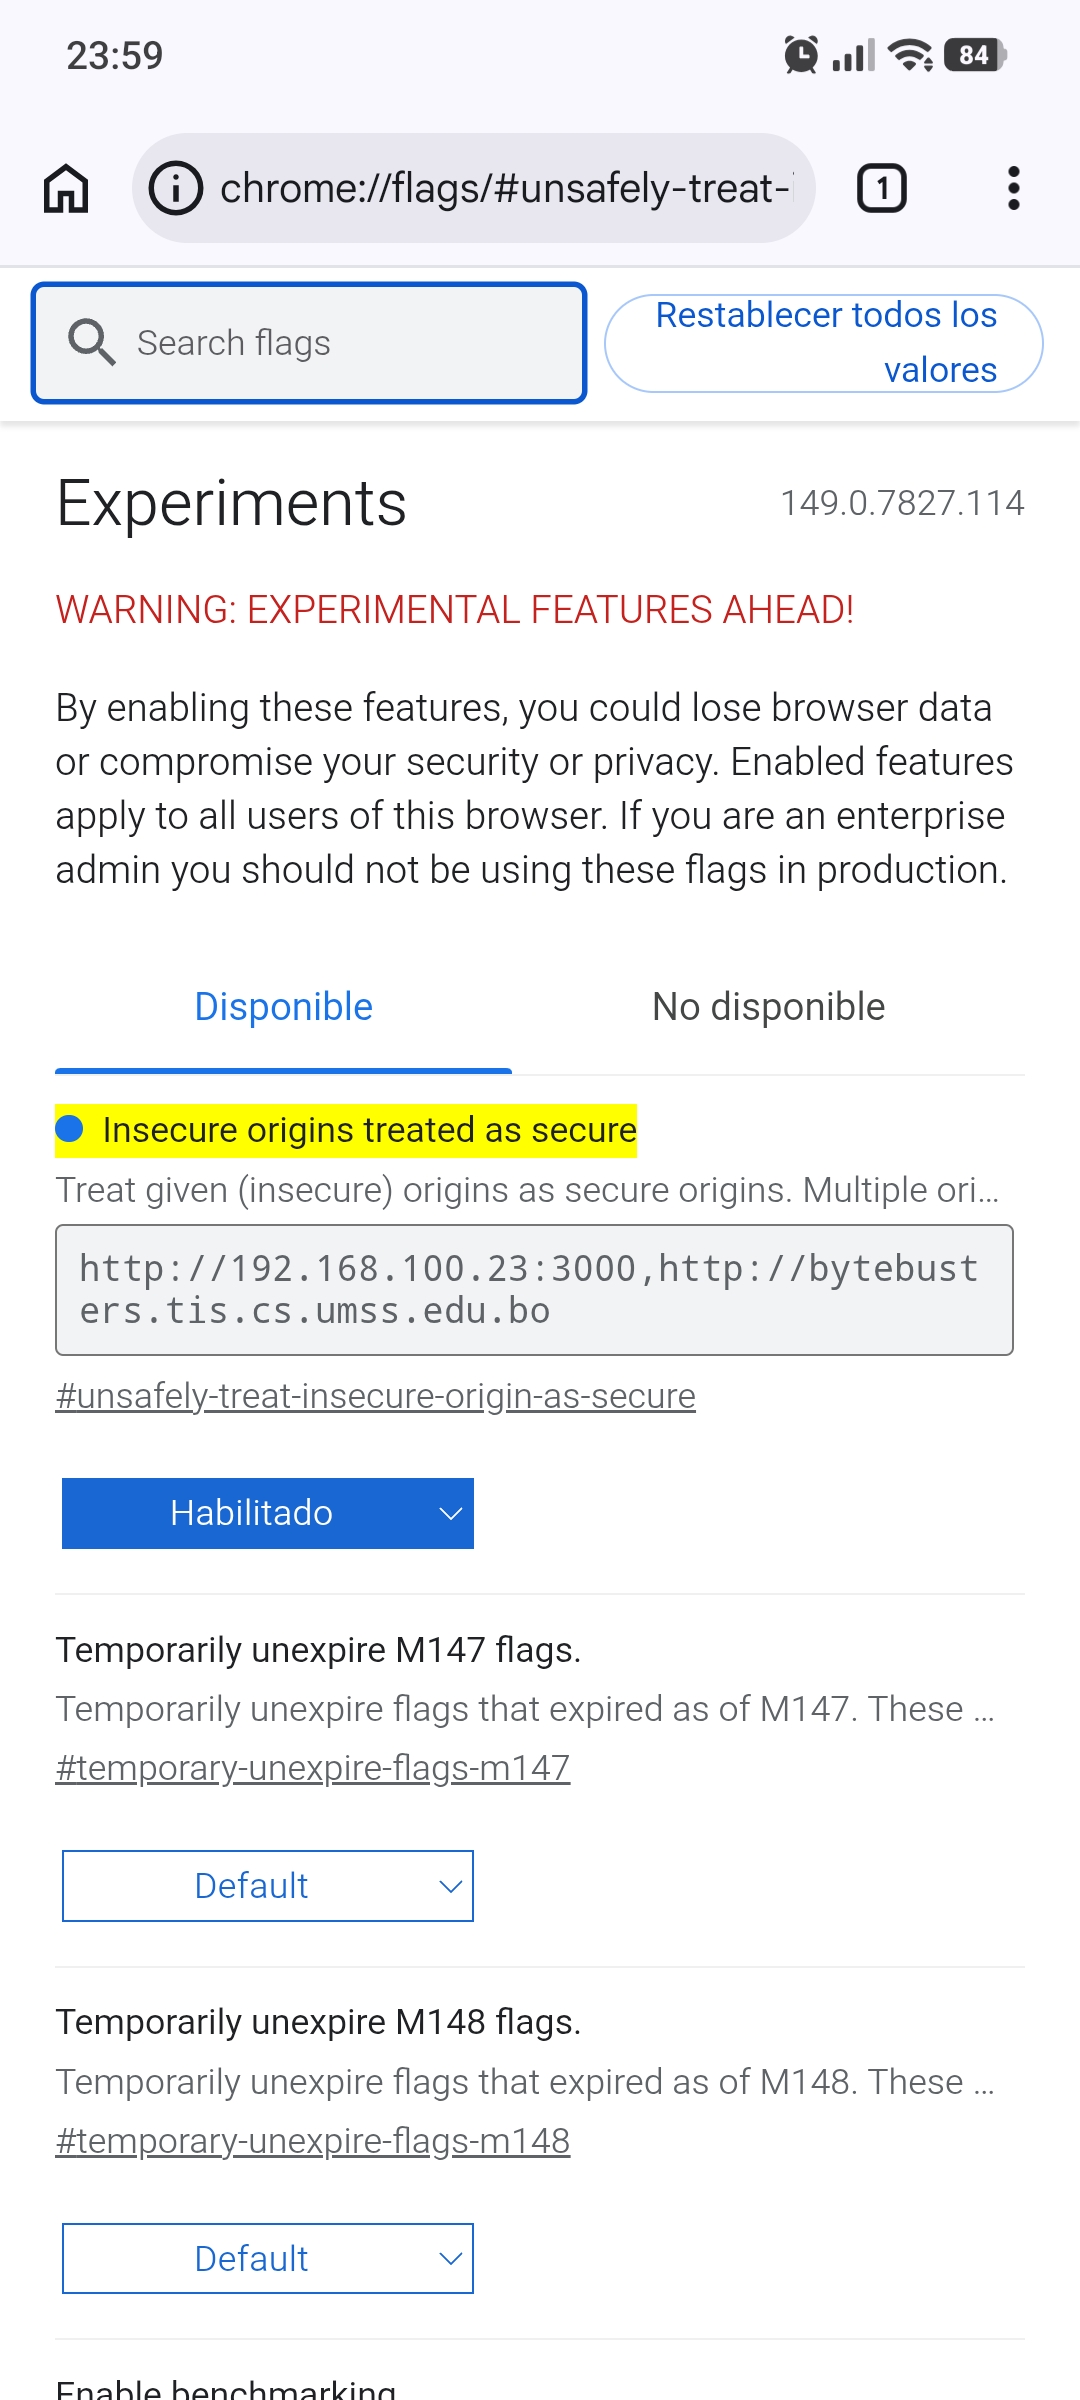
\includegraphics[width=0.35\linewidth]{assets/img/ethoshub/chromephone.jpg}
\caption{Página \texttt{chrome://flags} en Google Chrome Android, con la bandera «Insecure origins treated as secure» en \textit{Enabled} y los orígenes de confianza declarados.}%
\label{fig:chrome-android-flag}
\end{figure}

\begin{NotaConfiguracion}
En Android intervienen \textbf{dos} niveles de permiso: el de la \textit{bandera} del
navegador (que autoriza el origen inseguro) y el del \textbf{sistema operativo} (que
autoriza a la app de Chrome a usar la cámara). Ambos deben concederse. Si la cámara sigue
sin funcionar tras la bandera, revise los permisos de la app en los Ajustes de Android.
\end{NotaConfiguracion}

\subsection[Brave Browser (Escritorio y Android)]{Configuración de Navegadores basados en Chromium con Directivas Especiales (Brave Browser)}%
\label{subsec:brave}

Al estar construido sobre el motor de código abierto Chromium, Brave comparte las
directivas internas de control de hardware de Chrome, modificando exclusivamente el
protocolo del espacio de nombres de la aplicación (\comando{brave://} en lugar de
\comando{chrome://}).\par

\clearpage
\paragraph{En computadora de escritorio.}
\begin{enumerate}[noitemsep]
    \item Abra Brave y escriba en la barra de direcciones la ruta de banderas; pulse \textit{Enter}:\par
    \dir{brave://flags/\#unsafely-treat-insecure-origin-as-secure}
    \item Localice \textbf{«Insecure origins treated as secure»} y cambie su valor a \textbf{Enabled}.
    \item En el campo de texto que se habilita, pegue los orígenes objetivo separados por comas:\par
    \dir{http://192.168.100.23:3000,http://bytebusters.tis.cs.umss.edu.bo}
    \item Pulse \textbf{Relaunch} en la notificación inferior para reiniciar el navegador.
\end{enumerate}

\begin{figure}[htbp]
\centering
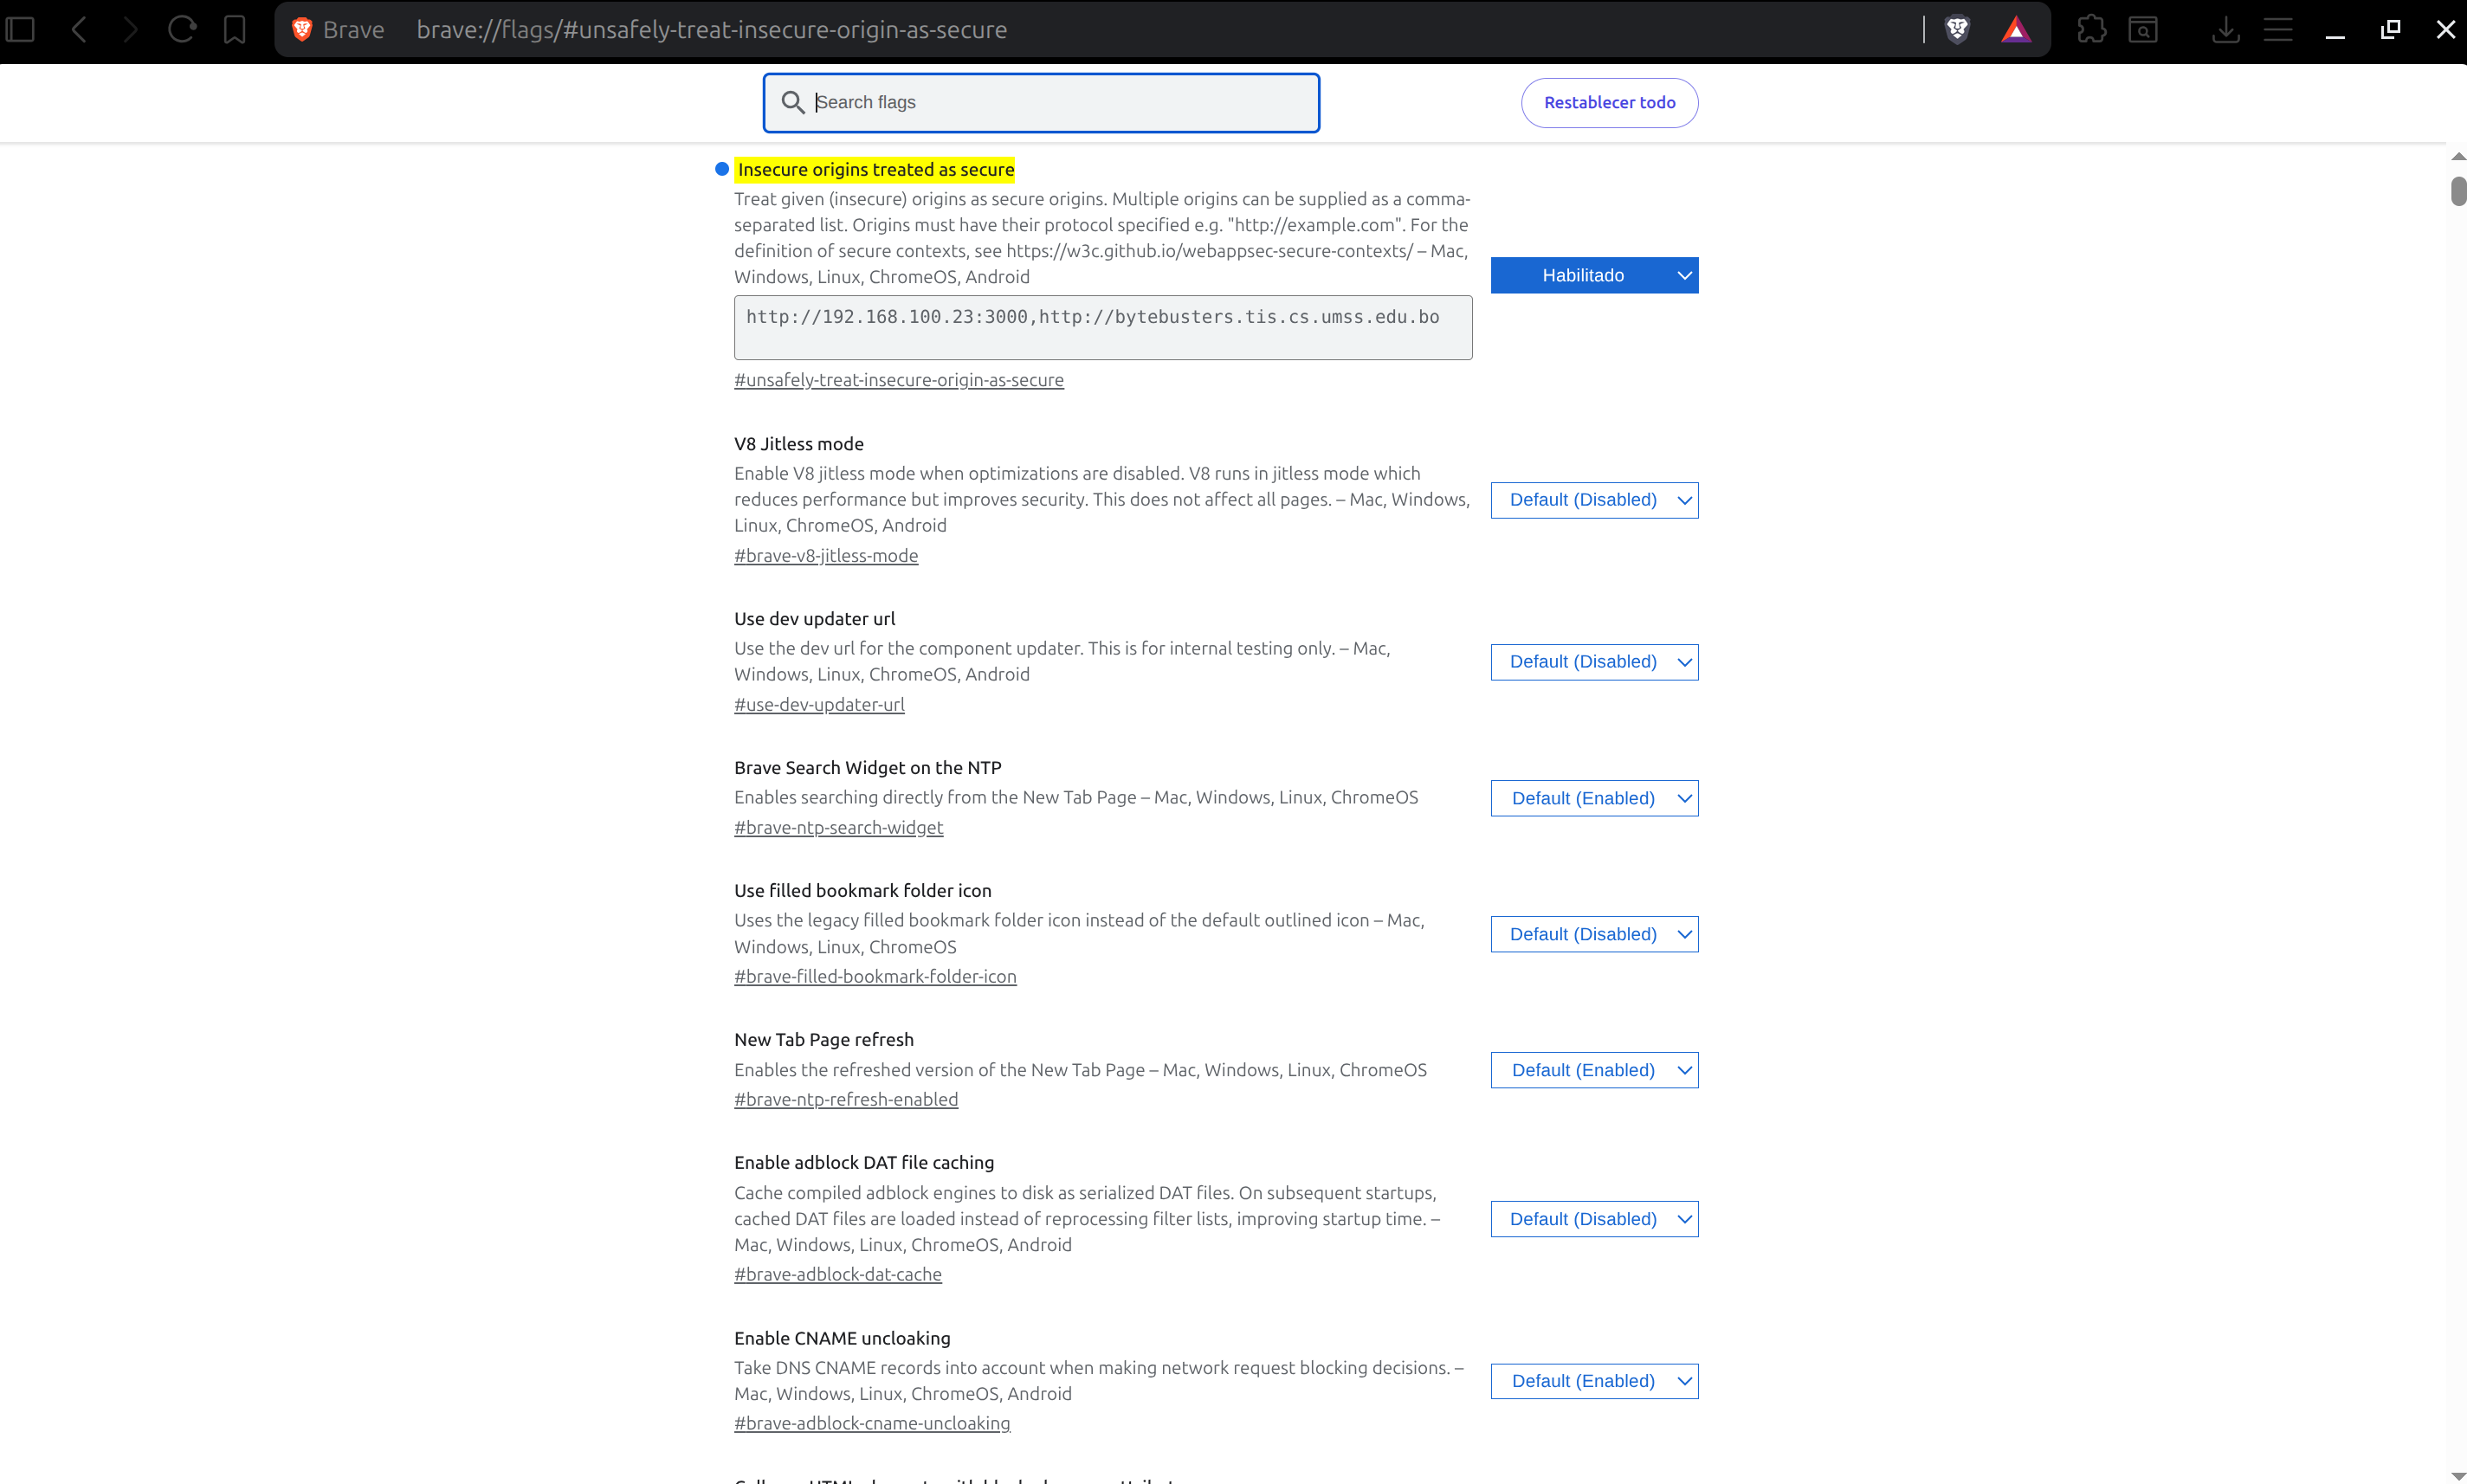
\includegraphics[width=0.85\linewidth]{assets/img/ethoshub/brave.png}
\caption{Página \texttt{brave://flags} en Brave de escritorio, con la bandera «Insecure origins treated as secure» en \textit{Enabled} y los orígenes de confianza declarados.}%
\label{fig:brave-pc-flag}
\end{figure}

\paragraph{En teléfono o tableta Android.}
\begin{enumerate}[noitemsep]
    \item Abra la app de Brave y escriba en la barra de direcciones la ruta \dir{brave://flags}; toque «Ir».
    \item Busque \comando{insecure} y abra \textbf{«Insecure origins treated as secure»}.
    \item Seleccione \textbf{Enabled} e introduzca los mismos orígenes separados por comas:\par
    \dir{http://192.168.100.23:3000,http://bytebusters.tis.cs.umss.edu.bo}
    \item Toque \textbf{Relaunch} para reiniciar Brave.
    \item Conceda el permiso de cámara/micrófono en el diálogo del sistema Android; si lo rechazó, habilítelo en \\ \comando{Ajustes $\to$ Aplicaciones $\to$ Brave $\to$ Permisos}.
\end{enumerate}

\clearpage
\begin{figure}[htbp]
\centering
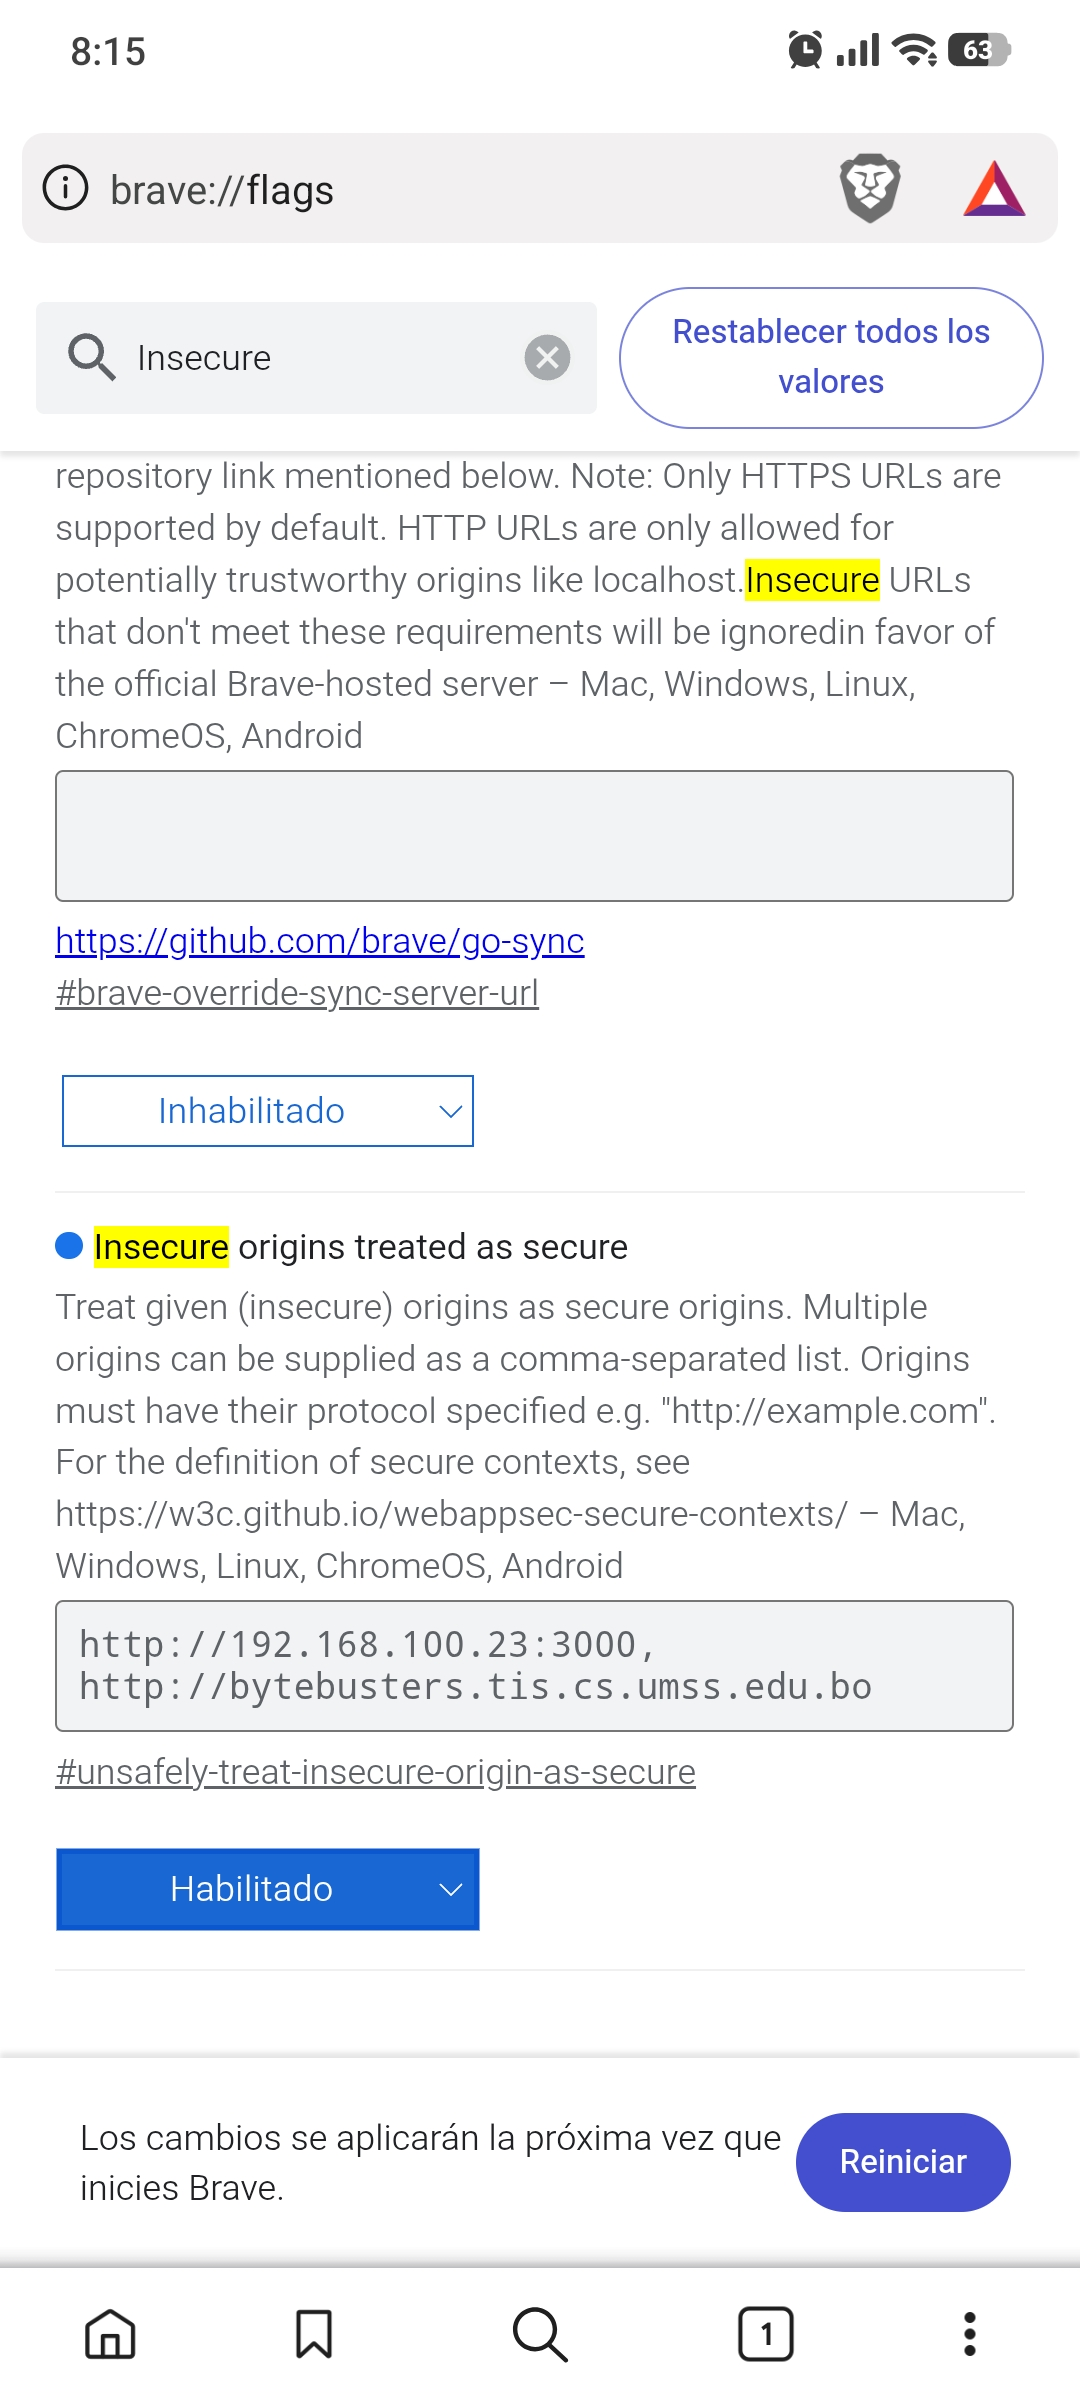
\includegraphics[width=0.35\linewidth]{assets/img/ethoshub/bravephone.jpg}
\caption{Página \texttt{brave://flags} en Brave Android, con la bandera «Insecure origins treated as secure» en \textit{Enabled} y los orígenes de confianza declarados.}%
\label{fig:brave-phone-flag}
\end{figure}

\subsection[Microsoft Edge (Escritorio y Android)]{Configuración de Directivas de Orígenes de Confianza en Microsoft Edge}%
\label{subsec:edge}

Las versiones actuales de Microsoft Edge se ejecutan bajo la misma plataforma base de
renderizado (Chromium), permitiendo la inyección de excepciones perimetrales de seguridad
de manera idéntica, mediante el espacio de nombres \comando{edge://}.\par

\paragraph{En computadora de escritorio.}
\begin{enumerate}[noitemsep]
    \item Abra Microsoft Edge y escriba en la barra de direcciones la ruta de banderas; pulse \textit{Enter}:\par
    \dir{edge://flags/\#unsafely-treat-insecure-origin-as-secure}
    \item Conmute el selector de \textbf{«Insecure origins treated as secure»} a \textbf{Enabled}.
    \item Inserte la lista de direcciones IP y dominios del proyecto separados por comas:\par
    \dir{http://192.168.100.23:3000,http://bytebusters.tis.cs.umss.edu.bo}
    \item Pulse \textbf{Restart} (Reiniciar) para actualizar los privilegios de captura de hardware.
\end{enumerate}

\clearpage
\paragraph{En teléfono o tableta Android.}
\begin{enumerate}[noitemsep]
    \item Abra la app de Edge y escriba \dir{edge://flags} en la barra de direcciones; toque «Ir».
    \item Busque \comando{insecure}, abra la opción y seleccione \textbf{Enabled}.
    \item Introduzca los mismos orígenes separados por comas:\par
    \dir{http://192.168.100.23:3000,http://bytebusters.tis.cs.umss.edu.bo}
    \item Toque \textbf{Restart} y, al volver, conceda el permiso de cámara/micrófono del sistema Android (o habilítelo en \comando{Ajustes $\to$ Aplicaciones $\to$ Edge $\to$ Permisos}).
\end{enumerate}

\begin{figure}[htbp]
\centering
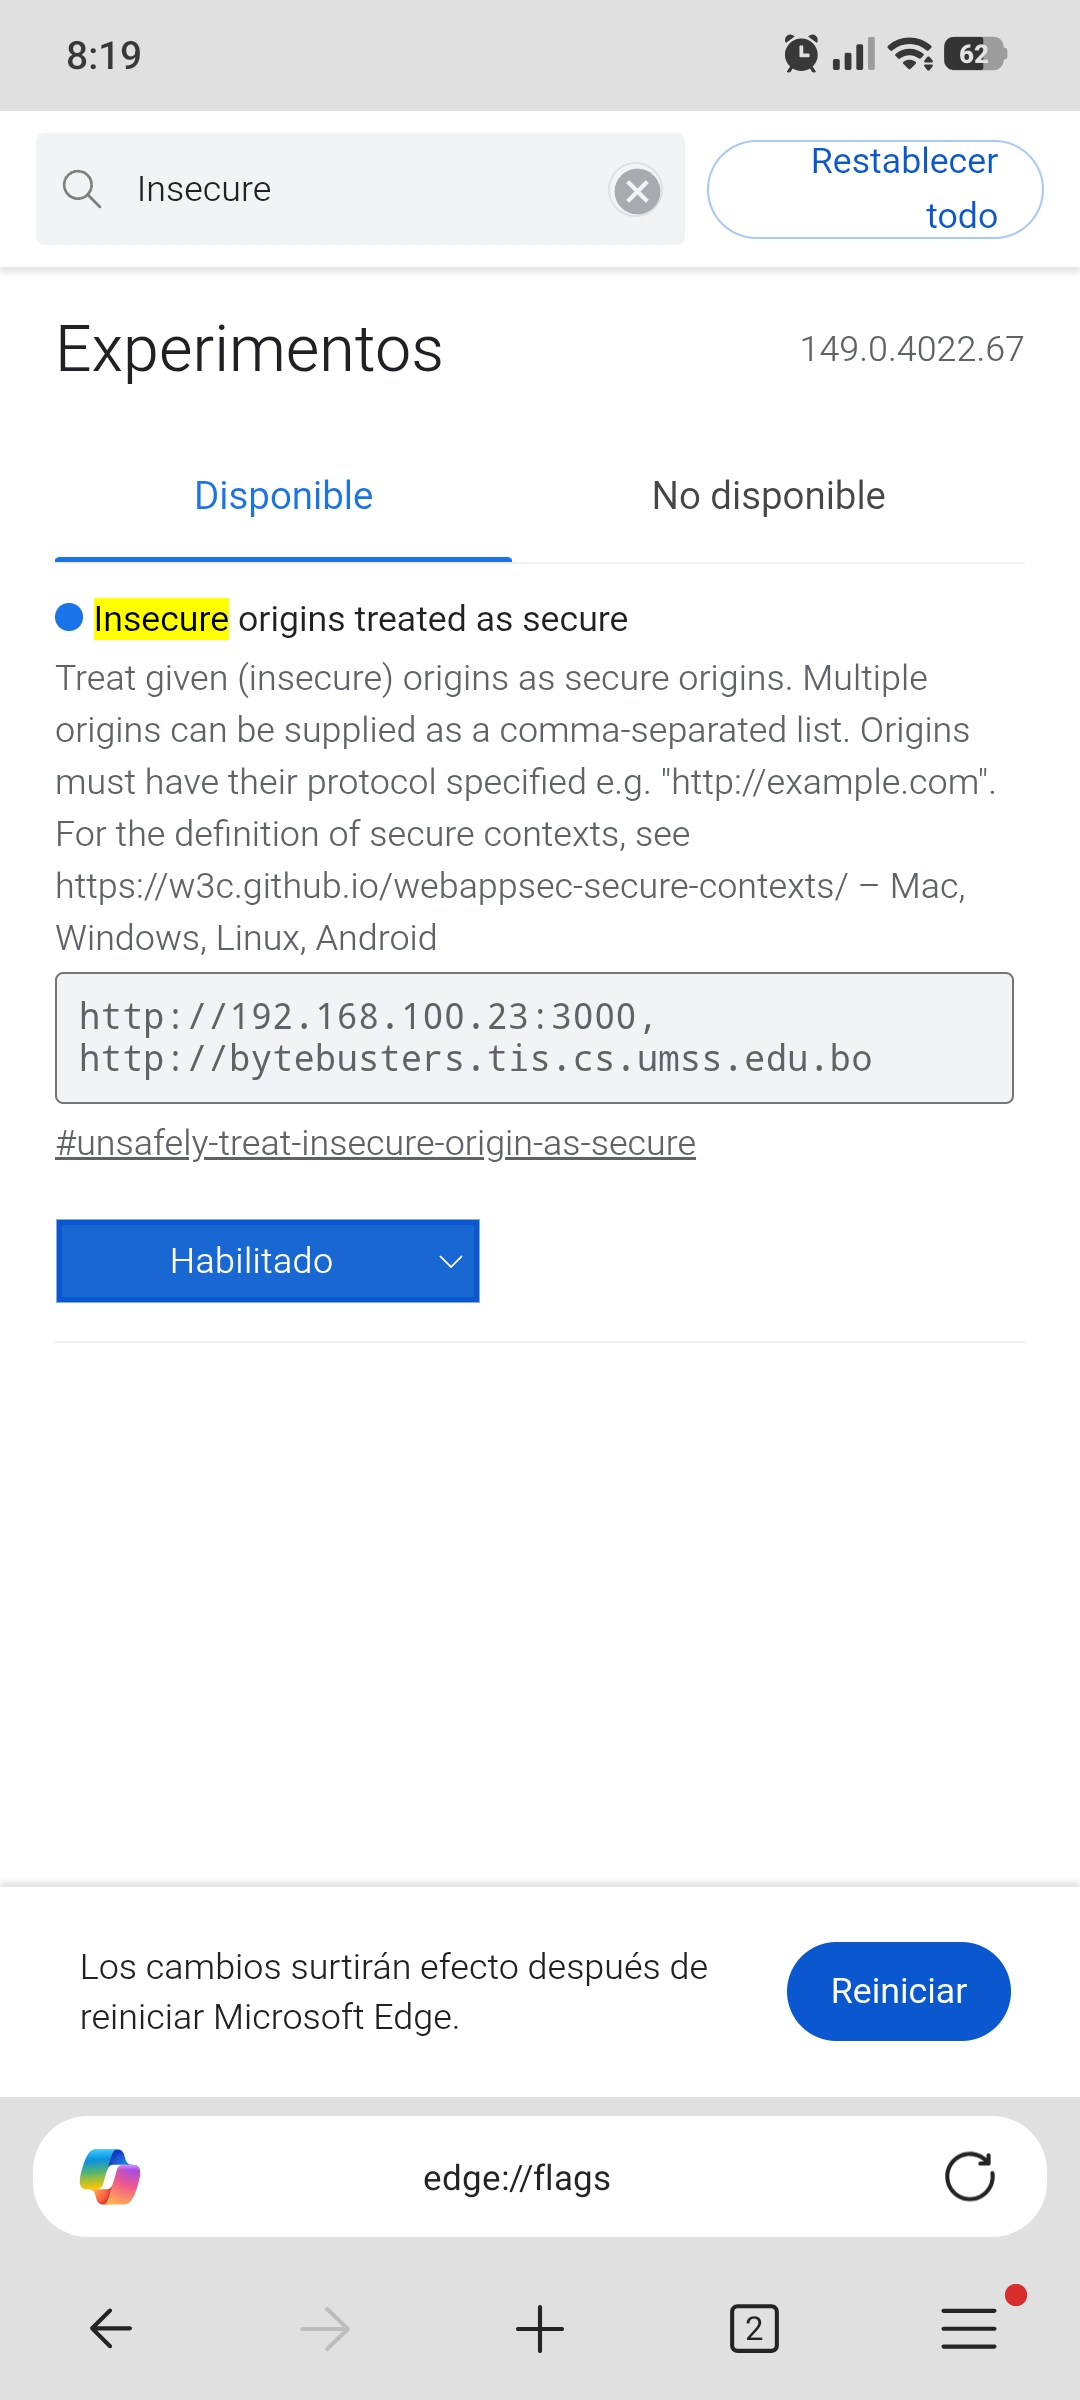
\includegraphics[width=0.35\linewidth]{assets/img/ethoshub/edgephone.jpg}
\caption{Página \texttt{edge://flags} en Microsoft Edge Android, con la bandera «Insecure origins treated as secure» en \textit{Enabled} y los orígenes de confianza declarados.}%
\label{fig:edge-phone-flag}
\end{figure}

\subsection[Mozilla Firefox (solo Escritorio)]{Configuración del Motor Gecko y Panel Interno de Preferencias en Escritorio (Mozilla Firefox)}%
\label{subsec:firefox}

El navegador Mozilla Firefox funciona bajo el motor independiente Gecko. Este entorno no
implementa el sistema tradicional de banderas individuales de Chromium, sino un entorno
unificado de variables globales avanzadas. Este procedimiento es aplicable exclusivamente
en computadoras personales (PC), puesto que las distribuciones móviles estándar de Firefox
bloquean el acceso de edición a esta capa de servicios.\par

\paragraph{En computadora de escritorio (único entorno admitido).}
\begin{enumerate}[noitemsep]
    \item Diríjase a la barra de direcciones e ingrese la instrucción de consola: \comando{about:config}
    \item Ante el mensaje de advertencia de seguridad del sistema, haga clic sobre la opción \textbf{«Aceptar el riesgo y continuar»}.
    \item En la barra superior de filtrado y búsqueda, introduzca exactamente la siguiente directiva: \\ \comando{media.devices.insecure.enabled}
    \item Por defecto, esta propiedad se encuentra en un estado lógico de \comando{false}. Ejecute una acción de doble clic sobre la línea (o presione el botón de inversión a la derecha) para conmutar su estado final a \textbf{true}.
    \item Realice una nueva búsqueda para la siguiente regla complementaria: \\ \comando{media.getusermedia.insecure.enabled}
    \item Modifique del mismo modo su valor para establecerlo firmemente en \textbf{true}.
    \item Cierre la pestaña actual, apague todas las instancias activas del navegador y reinicie el programa manualmente. Una vez completado, el motor otorgará acceso explícito a la cámara y micrófono bajo los dominios de prueba configurados.
\end{enumerate}

\begin{figure}[htbp]
\centering
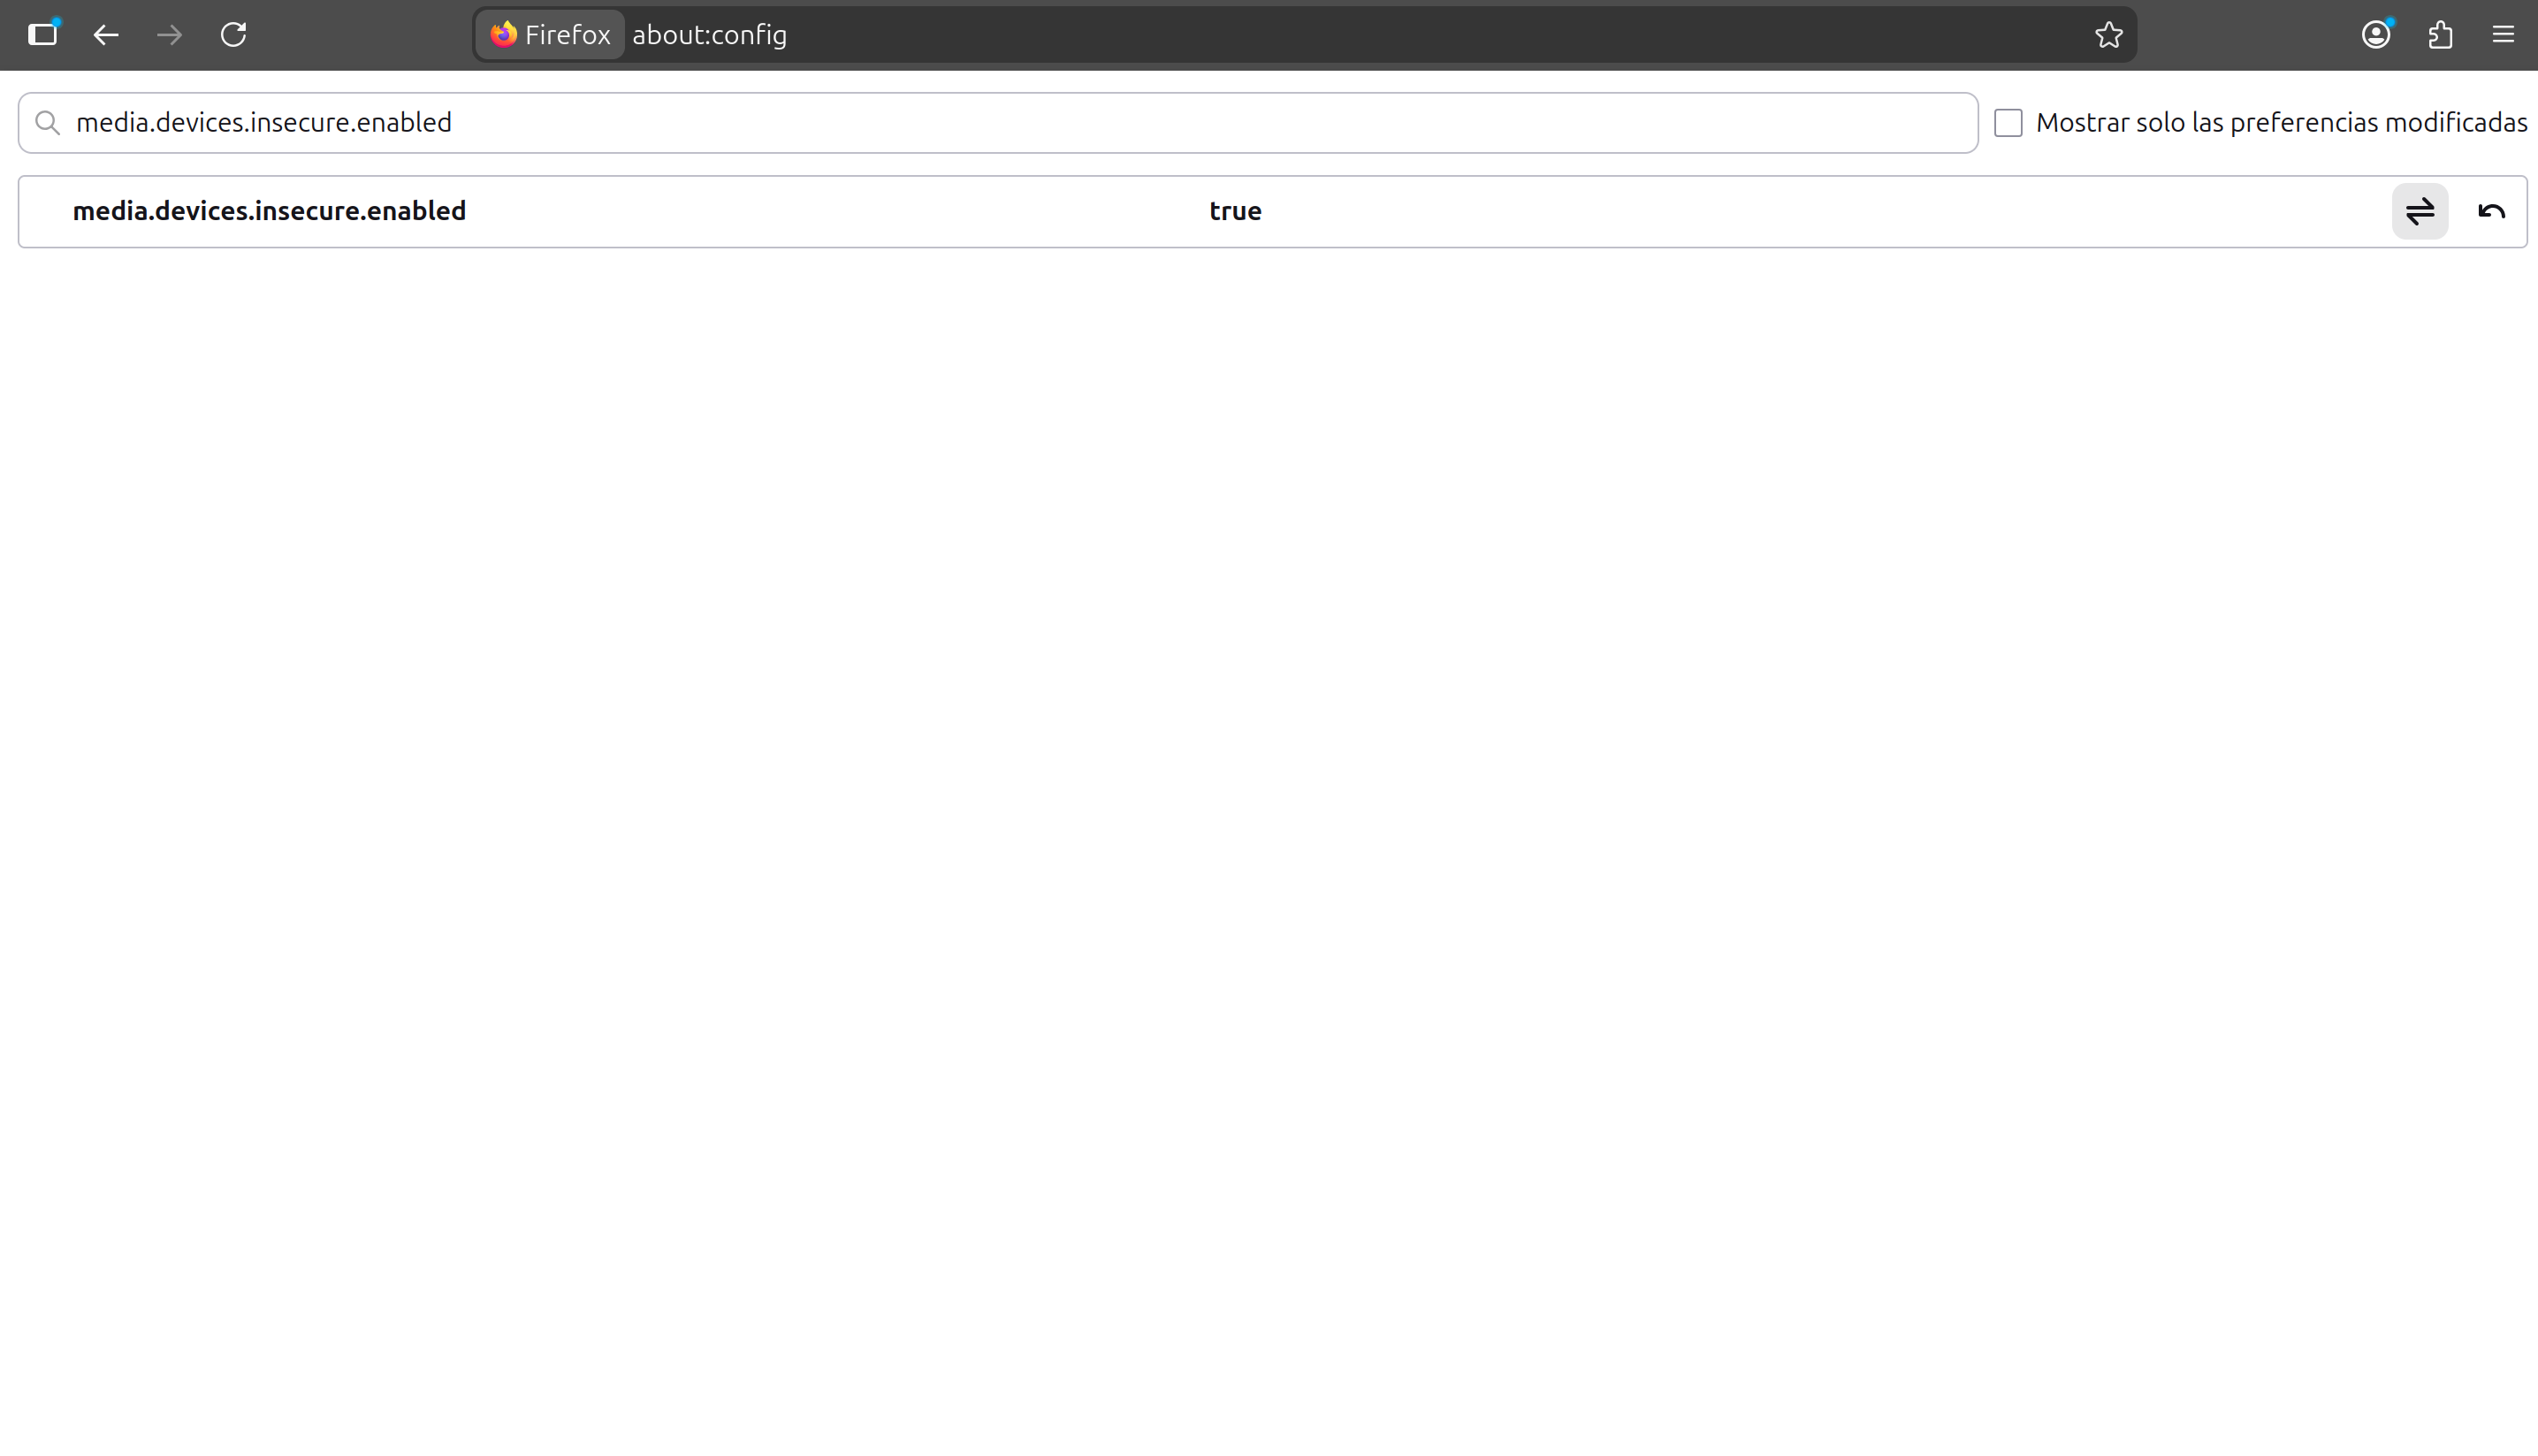
\includegraphics[width=0.85\linewidth]{assets/img/ethoshub/firefox.png}
\caption{Página \texttt{about:config} en Mozilla Firefox de escritorio, con las directivas «media.devices.insecure.enabled» y «media.getusermedia.insecure.enabled» en \textit{true} y los orígenes de confianza declarados.}%
\label{fig:firefox-pc-flag}
\end{figure}

\begin{AvisoAdvertencia}
\textbf{Firefox para Android no admite este procedimiento.} La versión móvil de Firefox no
expone las claves \comando{media.devices.insecure.enabled} ni
\comando{media.getusermedia.insecure.enabled} para su edición. En dispositivos Android que
deban usar la cámara/micrófono, emplee \textbf{Chrome, Brave o Edge} (apartados anteriores)
o sirva la aplicación bajo HTTPS.
\end{AvisoAdvertencia}

\par\vspace{0.2cm}
La tabla~\ref{tab:resumen-navegadores} resume, a modo de referencia rápida, la directiva y
el valor que debe aplicarse en cada navegador, junto con su soporte en Android.\par

\vspace{0.2cm}
\noindent
\renewcommand{\arraystretch}{1.35}
\fontsize{8.5}{10.2}\selectfont\sffamily
\begin{tabularx}{\dimexpr\textwidth-2pt\relax}{|>{\bfseries\color{colorPrimario}}l|>{\ttfamily\raggedright\arraybackslash\fontsize{7.6}{9}\selectfont}p{4.7cm}|>{\raggedright\arraybackslash}X|c|}
\hline
\rowcolor{headerTabla}
\sffamily\textbf{Navegador} & \sffamily\textbf{Directiva} & \sffamily\textbf{Valor} & \sffamily\textbf{Android} \\
\hline
Google Chrome & \seqsplit{chrome://flags/\#unsafely-treat-insecure-origin-as-secure} & Enabled + orígenes & Sí \\
\hline
\rowcolor{grisTecnico}
Brave & \seqsplit{brave://flags/\#unsafely-treat-insecure-origin-as-secure} & Enabled + orígenes & Sí \\
\hline
Microsoft Edge & \seqsplit{edge://flags/\#unsafely-treat-insecure-origin-as-secure} & Enabled + orígenes & Sí \\
\hline
\rowcolor{grisTecnico}
Mozilla Firefox & \seqsplit{media.devices.insecure.enabled} \newline \seqsplit{media.getusermedia.insecure.enabled} & true \newline true & No \\
\hline
\end{tabularx}\normalfont\normalsize%
\label{tab:resumen-navegadores}

\begin{VerificacionOK}
Tras reiniciar el navegador, acceda al CV Studio y active la captura de vídeo. El navegador
debe solicitar permiso de cámara/micrófono (en lugar de bloquearlo silenciosamente). Si lo
solicita y, al conceder, la previsualización se muestra, la excepción de origen está
correctamente aplicada.
\end{VerificacionOK}

\par\vspace{0.2cm}
Con la seguridad configurada, el capítulo~\ref{ch:verificacion} establece el protocolo para
verificar que la instalación es plenamente funcional.\par
